\documentclass[a4paper,oneside,12pt]{article}

\usepackage[utf8x]{inputenc}
\usepackage[T1]{fontenc}
\usepackage{hyperref}
\usepackage{eurosym}
\usepackage{graphicx}
\usepackage{array}
\newcolumntype{C}{>{\centering\arraybackslash}p{8ex}}
\usepackage[binary-units = true]{siunitx}

\title{TASBot64\\Specifications}
\author{rcavadas, abureau,\\cmutti, lgillot-}

\begin{document}
\maketitle

\section{Functional purpose}
The TASBot64 is a device that plugs in a Nintendo 64 to play a pre-recorded Tool
Assisted Speedrun (TAS) input file, faking a gamepad.

A TAS is a speedrun (the completion of a video game in the shortest time
possible) whose inputs, that is to say the sequence of buttons pressing and
movements on the gamepad, are given frame-by-frame on an emulator.

Emulators enable techniques such as frame-by-frame operation, precise digital
and analog inputs, re-recording (saving and reloading the entire state of the
game at any moment) or even memory watching and disassembly.

Thanks to this, TASs showcase feats unattainable to the human player and often
feature blatant abuse of the game mechanisms, exploiting bugs in the games that
was not intended to receive such fast and improbable input.

If the emulator is needed to craft the input file, the sequence of inputs itself
however is perfectly valid and theorically could come from a real gamepad. Hence
the goal of the TASBot64, that is to perform a TAS on a real Nintendo 64 instead
of an emulator, thus validating that the TAS does not depend on any emulator
specificity.

\subsection{Features}
\begin{itemize}
\item Behave as a genuine Nintendo 64 gamepad
\item Read and play the Mupen64-rr input file format from a SD card
\item Allow selecting between different files on the SD
\item Allow selecting between 50Hz (Europe) and 60Hz (US and Japan) operation
\item Display the name of the current selected file
\item Display errors or unsupported features if they occur
\item Allow passthrough of a gamepad to the console to avoid frequent unplugging
\item Take its power from the Nintendo 64 (no power source required)
\end{itemize}

\subsection{Performances}
\begin{itemize}
\item The user must be able to choose between 4 different input files
\item The TASBot64 must support input files as big as 4GB
\item The output stream to the console must be fast enough so as to not miss a
  game frame: a complete input frame must be emited in less than a 60th of a
  second.
\item The output stream rate must not drift more than half a frame (at most 8ms)
  in a runtime of 24 hours
\item The delay between startup of console and first output frame must be
  shorter than 0.5s and must not vary more than a quarter of a frame (at most
  4ms) between runs
\item The latency between input and output during passthrough must be less than
  1 ms
\end{itemize}

\section{User manual}
\subsection{Front panel}
The PCB itself presents on its control panel:
\begin{itemize}
\item A display. The backlight indicates is the TASBot64 is on. On the first line
  is shown the name of the TAS movie being played. On the second line is shown
  the progression of the TAS and any eventual error code
\item Two buttons, up and down, to cycle between TAS movies
\item A "Mode" switch which allows you to chose between "PASSTHROUGH" mode and
  "TAS" mode
\item The SD port where you can insert your SD card (non included).
\end{itemize}

\subsection{Connection}
The TASBot64 has got one gamepad input port and four gamepad output cables. Plug
a gamepad in the input port if you want to use the passthrough mode. Plug one to
four output cable into the Nintendo 64 depending on the game played.

\subsection{Reading a TAS}
\subsubsection{Getting files (Mupen64 movies)}
First of all, you have to download at least one and up to four files to be read
by your TASBot64 from the Internet to your SD card (not included). Such files
can be found on specialized websites such as tasvideos.org
Once the files are loaded, insert your SD card into the adapted slot of the
TASBot64.

Our tip: you may want to visit http://tasvideos.org/Movies-N64-Stars-Moons.html

Important: please notice that you must own the cartridge of the game you want to
run the TAS.

Important: please notice that only .m64 files (Mupen64 movies) can be read by
your TASBot64 so make sure to get these.

\subsubsection{Preparing the ground}
Every TAS has been created to run from a certain state of the game. You have to
put your game cartridge in this specific state in order to run the TAS you've
chosen. Generally this means deleting all data from the first file of the game
cartridge but THIS MAY VARY FOR SOME OF THEM. In any case, we recommend to
double check the TAS video (you will find links to these under the .m64 files on
tasvideos.org) before starting a run.

\subsubsection{Running the TAS}
\begin{itemize}
\item Put the appropriate game cartridge into your Nintendo 64 system
\item Connect your TASBot64 to the relevant controller port of your Nintendo 64
system
\item Switch the mode switch to TAS position
\item If the movie name on the display is the want you want to play, you have
  nothing to do but watch the TAS playing.
\item If the movie name isn't the one you want to play, choose another one with
  the up and down buttons. The TAS will stop playing until you reset the
  console. The TASBot64 will remember which movie you had selected.
\end{itemize}

\subsection{Passthrough mode}
When the mode switch is in passthrough mode, you can simply play your Nintendo
64 game, without needing to unplug the TASBot64 from the console and plug your
gamepad instead.

\subsection{Errors and how to fix them}
\subsubsection{TAS mode}
\begin{itemize}
\item TAS doesn't start: check if the mode switch is on TAS mode
\item TAS seems desynchronized: check if the TAS movie name on the screen is the
  right one, if not then select the right one using the up and down buttons and
  restart the Nintendo 64 system
\item TAS didn't finish the game: the game cartridge may not be at its correct
initial state or the TAS may be invalid.
\item You can't find your TAS movie: make sure the file has the .m64 extension
\end{itemize}

\subsubsection{Passthrough mode}
\begin{itemize}
\item The game seems to play by itself: check if the mode switch is on
Passthrough mode
\item I can't do anything : Check if the controller is properly connected
\end{itemize}

\subsubsection{Error Code}
\begin{itemize}
\item \texttt{NO\ SD}: insert a SD card in the adapted slot
\item \texttt{FS\ ERR}: error while parsing the file system, make sure your SD card has a
  partition table and is properly formatted
\item \texttt{NO\ FILE}: SD card is empty, load at least one file in your SD card
\item \texttt{PARSE\ ERR}: error while parsing the TAS movie file, make sure your .m64
  file is actually a Mupen64-rr movie file and is not corrupted
\item \texttt{NOEPAD}: Not enough output cables are plugged to the gamepad ports of the
  Nintendo 64 for this movie file.
\item \texttt{UNSUPP}: An unsupported feature of the Mupen64-rr movie format is present
  in the file you are playing, the movie cannot played anymore.
\end{itemize}

\section{Protocols}
\subsection{N64 to Gamepad}
\subsubsection{Electrical levels}
The gamepad is connected to the Nintendo 64 by a cable made of a \SI{3.3}{\V}
alim wire, a ground wire and a data wire.

This data wire is a bidirectionnal serial bus. It is operated in an open
collector way, pulled up to \SI{3.3}{\V}. Hence, both the console and the
gamepad can talk half-duplex on it by pulling down the line in a wire-AND
scheme.

As measured, the console pulls down the line to \SI0{\V}, while our gamepad
pulls it only down to \SI{655}{\mV}, probably due to a diode on the path.

\subsubsection{Bit signaling and framing}
Each bit of data on the wire is made of a falling edge followed by a rising
edge. What distinguish a 0 bit from a 1 bit is the duration of the low state, as
pictured in figures \ref{0bit} and \ref{1bit}.

\begin{figure}
  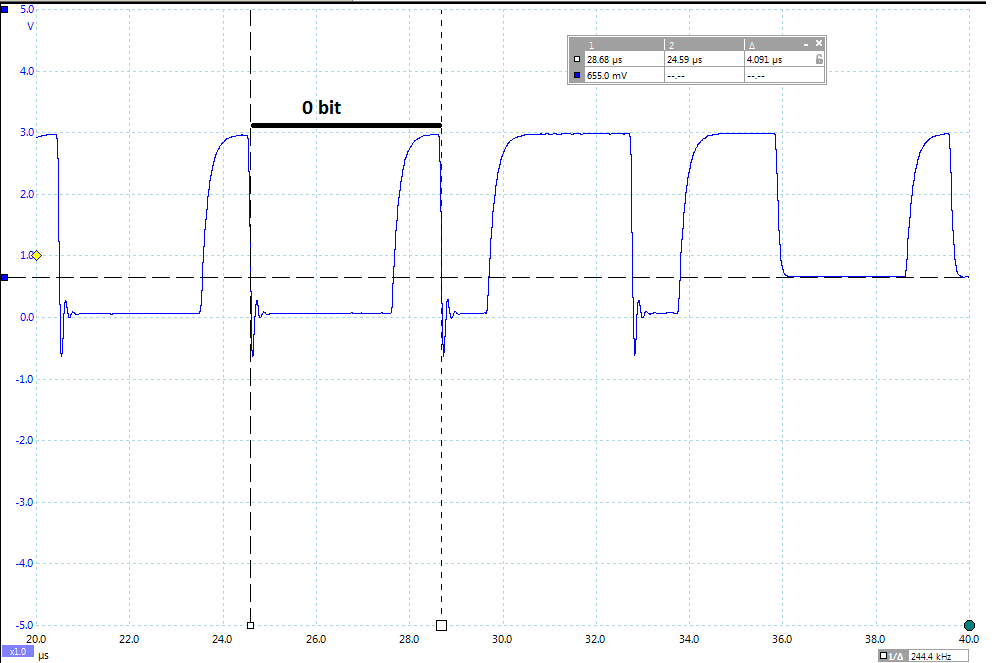
\includegraphics[width=\textwidth]{0bit.png}
  \caption{0 bit}
  \label{0bit}
\end{figure}

\begin{figure}
  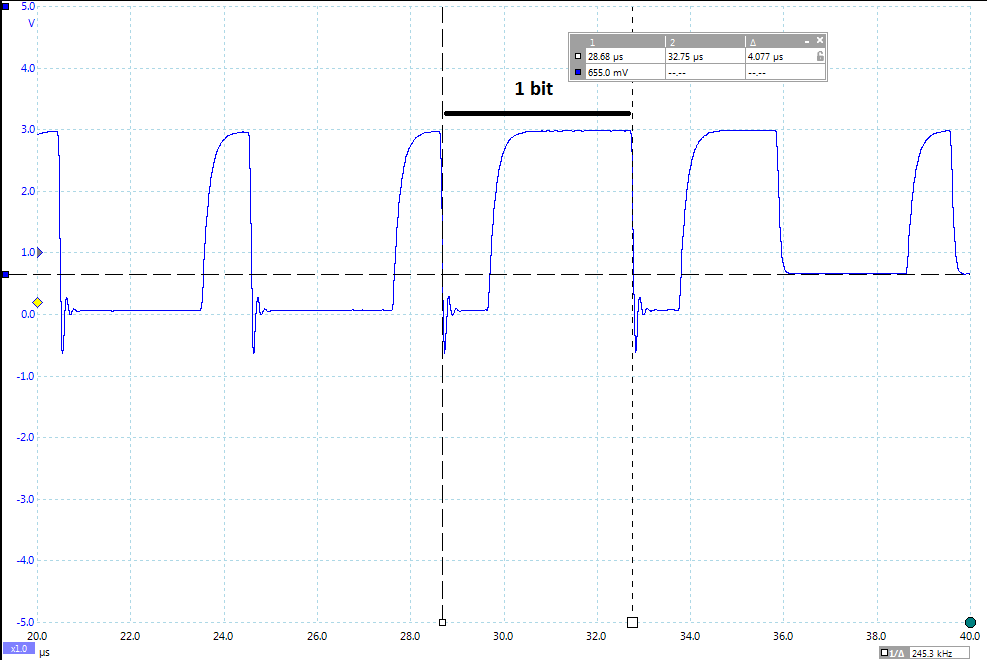
\includegraphics[width=\textwidth]{1bit.png}
  \caption{1 bit}
  \label{1bit}
\end{figure}

Communication is done in frames of 1 to 4 bytes. A frame starts directly with a
data bit. Each bit is separated of the next by a high state of at least
\SI{0.5}{\us}. After all bytes are transmitted, the frame ends with a last
falling edge and then the line is released.

\subsubsection{Input protocol}
The inputs are always transmitted on console demand: the gamepad never
spontaneously emit input information. When the console sends a request frame,
the gamepad sends back a frame containing the full state of the gamepad at the
moment. The total communication does not take longer than \SI{200}{\us}.

The console does not necessarily asks for input on a regular basis: a long time
could go between requests, for example if the game currently does not take
inputs at the moment or if it taking inputs from another gamepad. However the
console will not ask the same gamepad more than once in a frame time (at least
\SI{16}{\ms}).

The request frame is one 0b00000001 byte.
The response is a 4 byte frame representing the simultaneous inputs of the
paddle buttons and joystick, read as follow:

\begin{itemize}
\item Byte 0: see table \ref{byte0}
  \begin{table}
    \begin{tabular}{|*{8}{C|}}
      \hline
      \multicolumn{1}{|l}{7}&\multicolumn{6}{c}{}&\multicolumn{1}{r|}{0}\\
      \hline
      A&B&Z&Start&DPad up&DPad down&DPad left&DPad right\\
      \hline
    \end{tabular}
    \caption{Input byte 0}
    \label{byte0}
  \end{table}
\item Byte 1: see table \ref{byte1}
  \begin{table}
    \begin{tabular}{|*{8}{C|}}
      \hline
      \multicolumn{1}{|l}{7}&\multicolumn{6}{c}{}&\multicolumn{1}{r|}{0}\\
      \hline
      Reserved&Reserved&L&R&C up&C down &C left&C right\\
      \hline
    \end{tabular}
    \caption{Input byte 1}
    \label{byte1}
  \end{table}
\item Byte 2: Joystick X axis range from -128 (left position) to 127 (right
  position)
\item Byte 3: Joystick Y axis range from -128 (down position) to 127 (up position)
\end{itemize}

\begin{figure}
  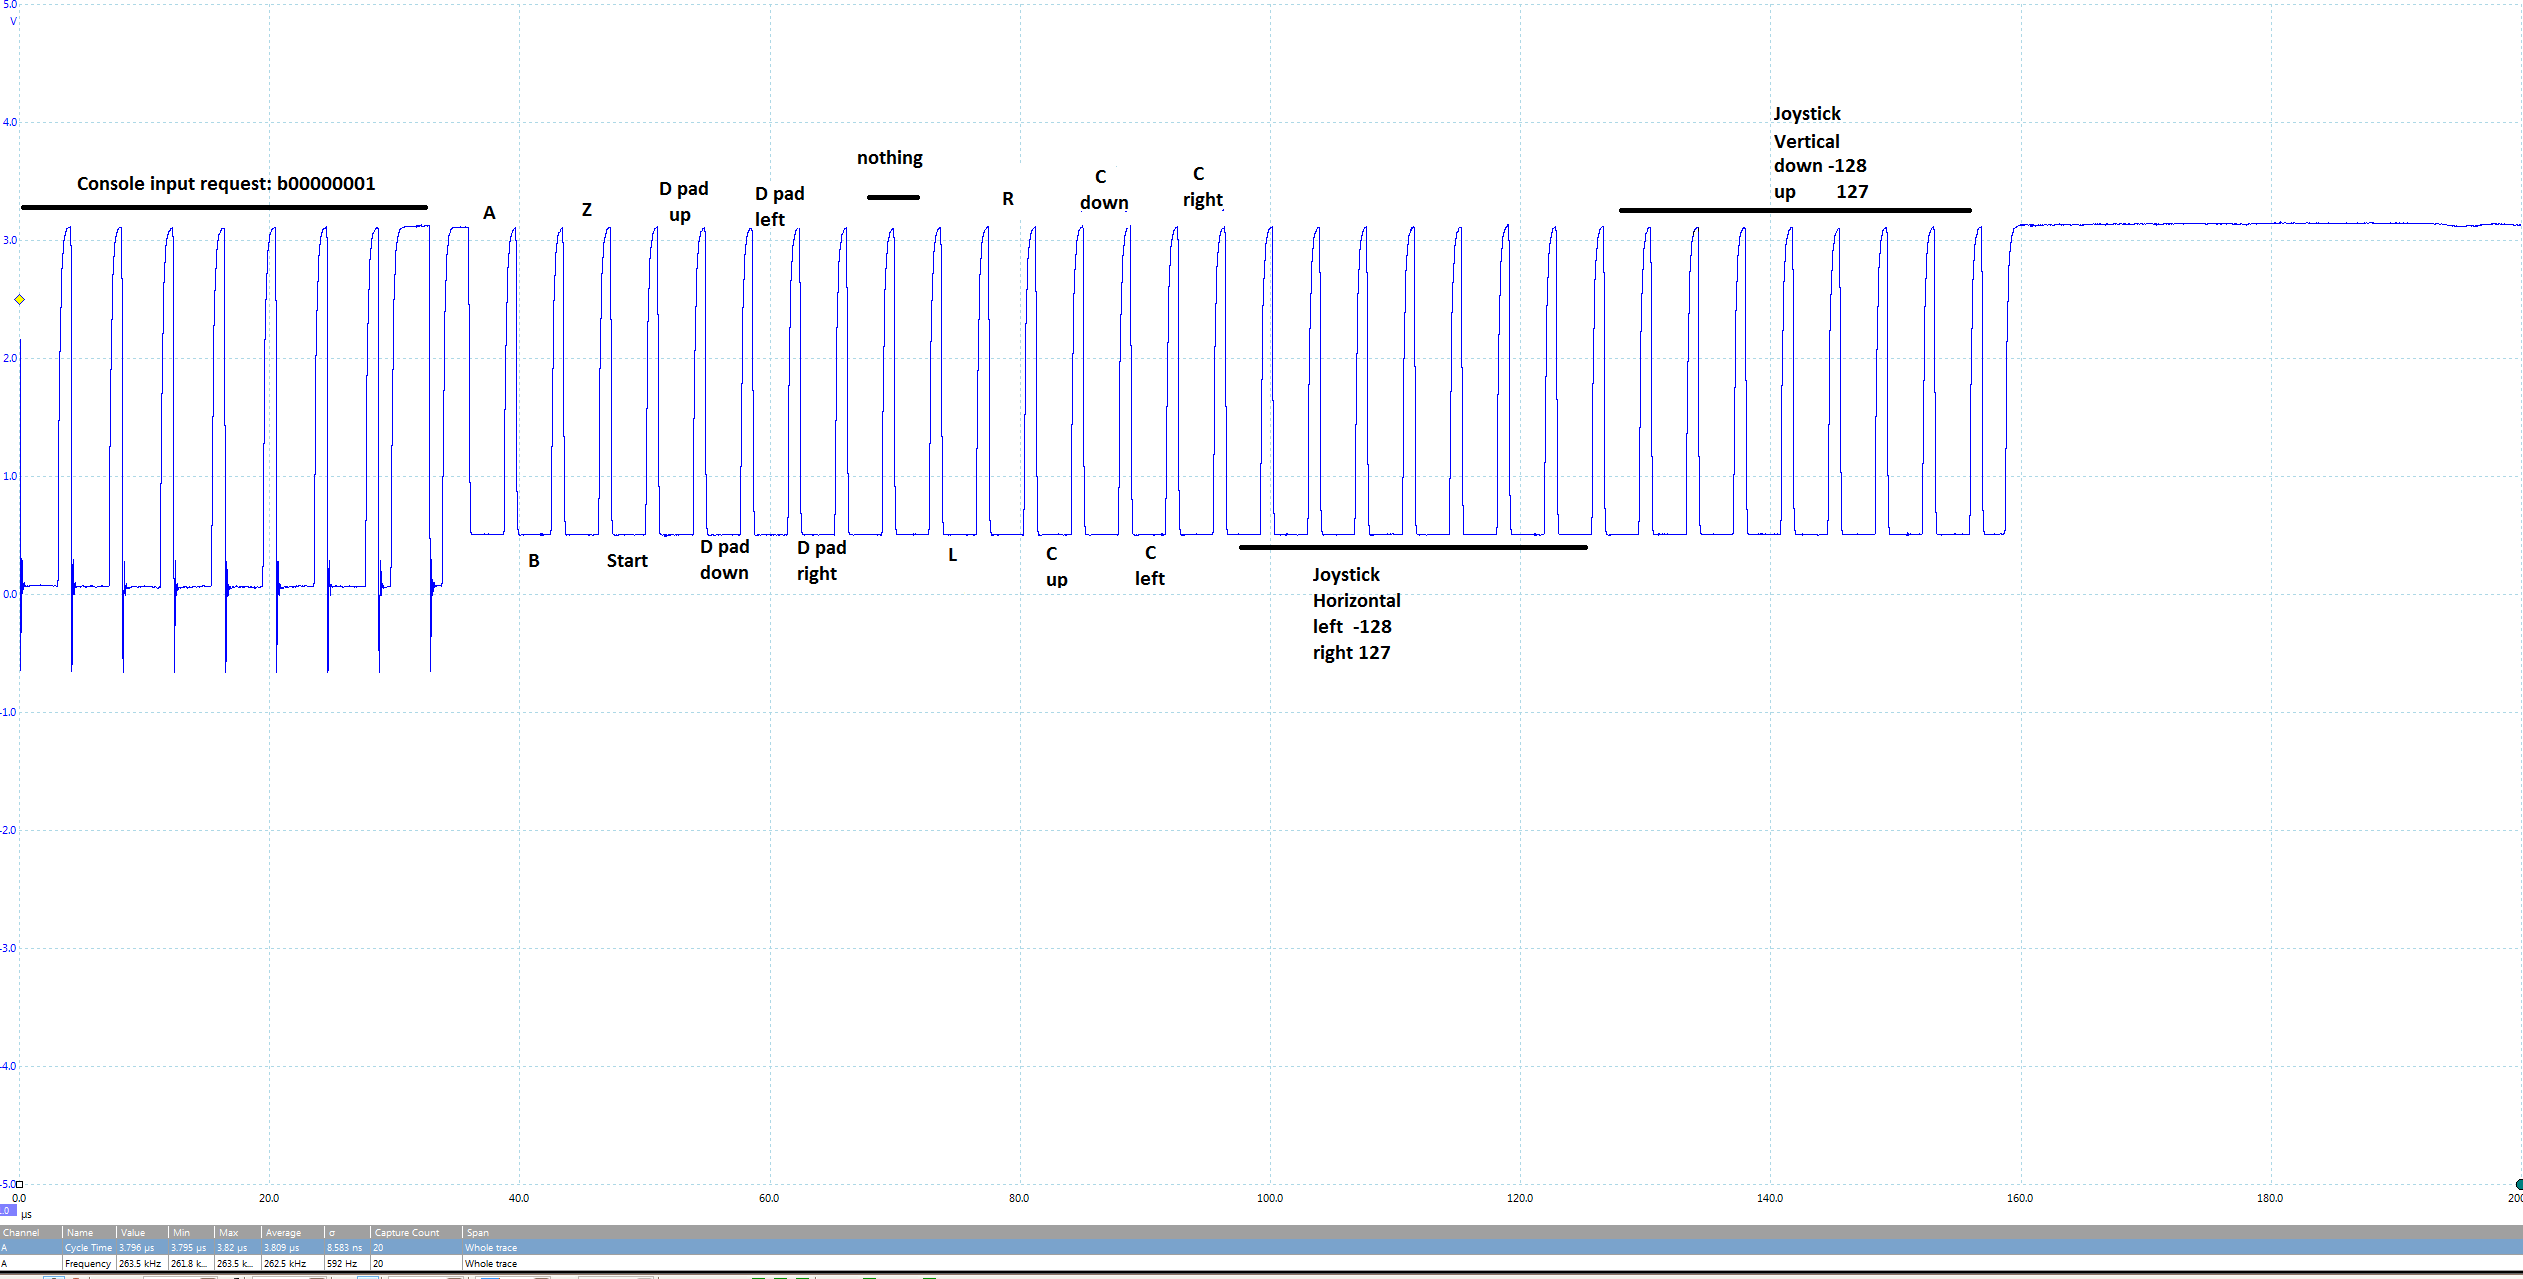
\includegraphics[width=\textwidth]{input_legend.png}
  \caption{Input bits meaning}
  \label{input_legend}
\end{figure}

\begin{figure}
  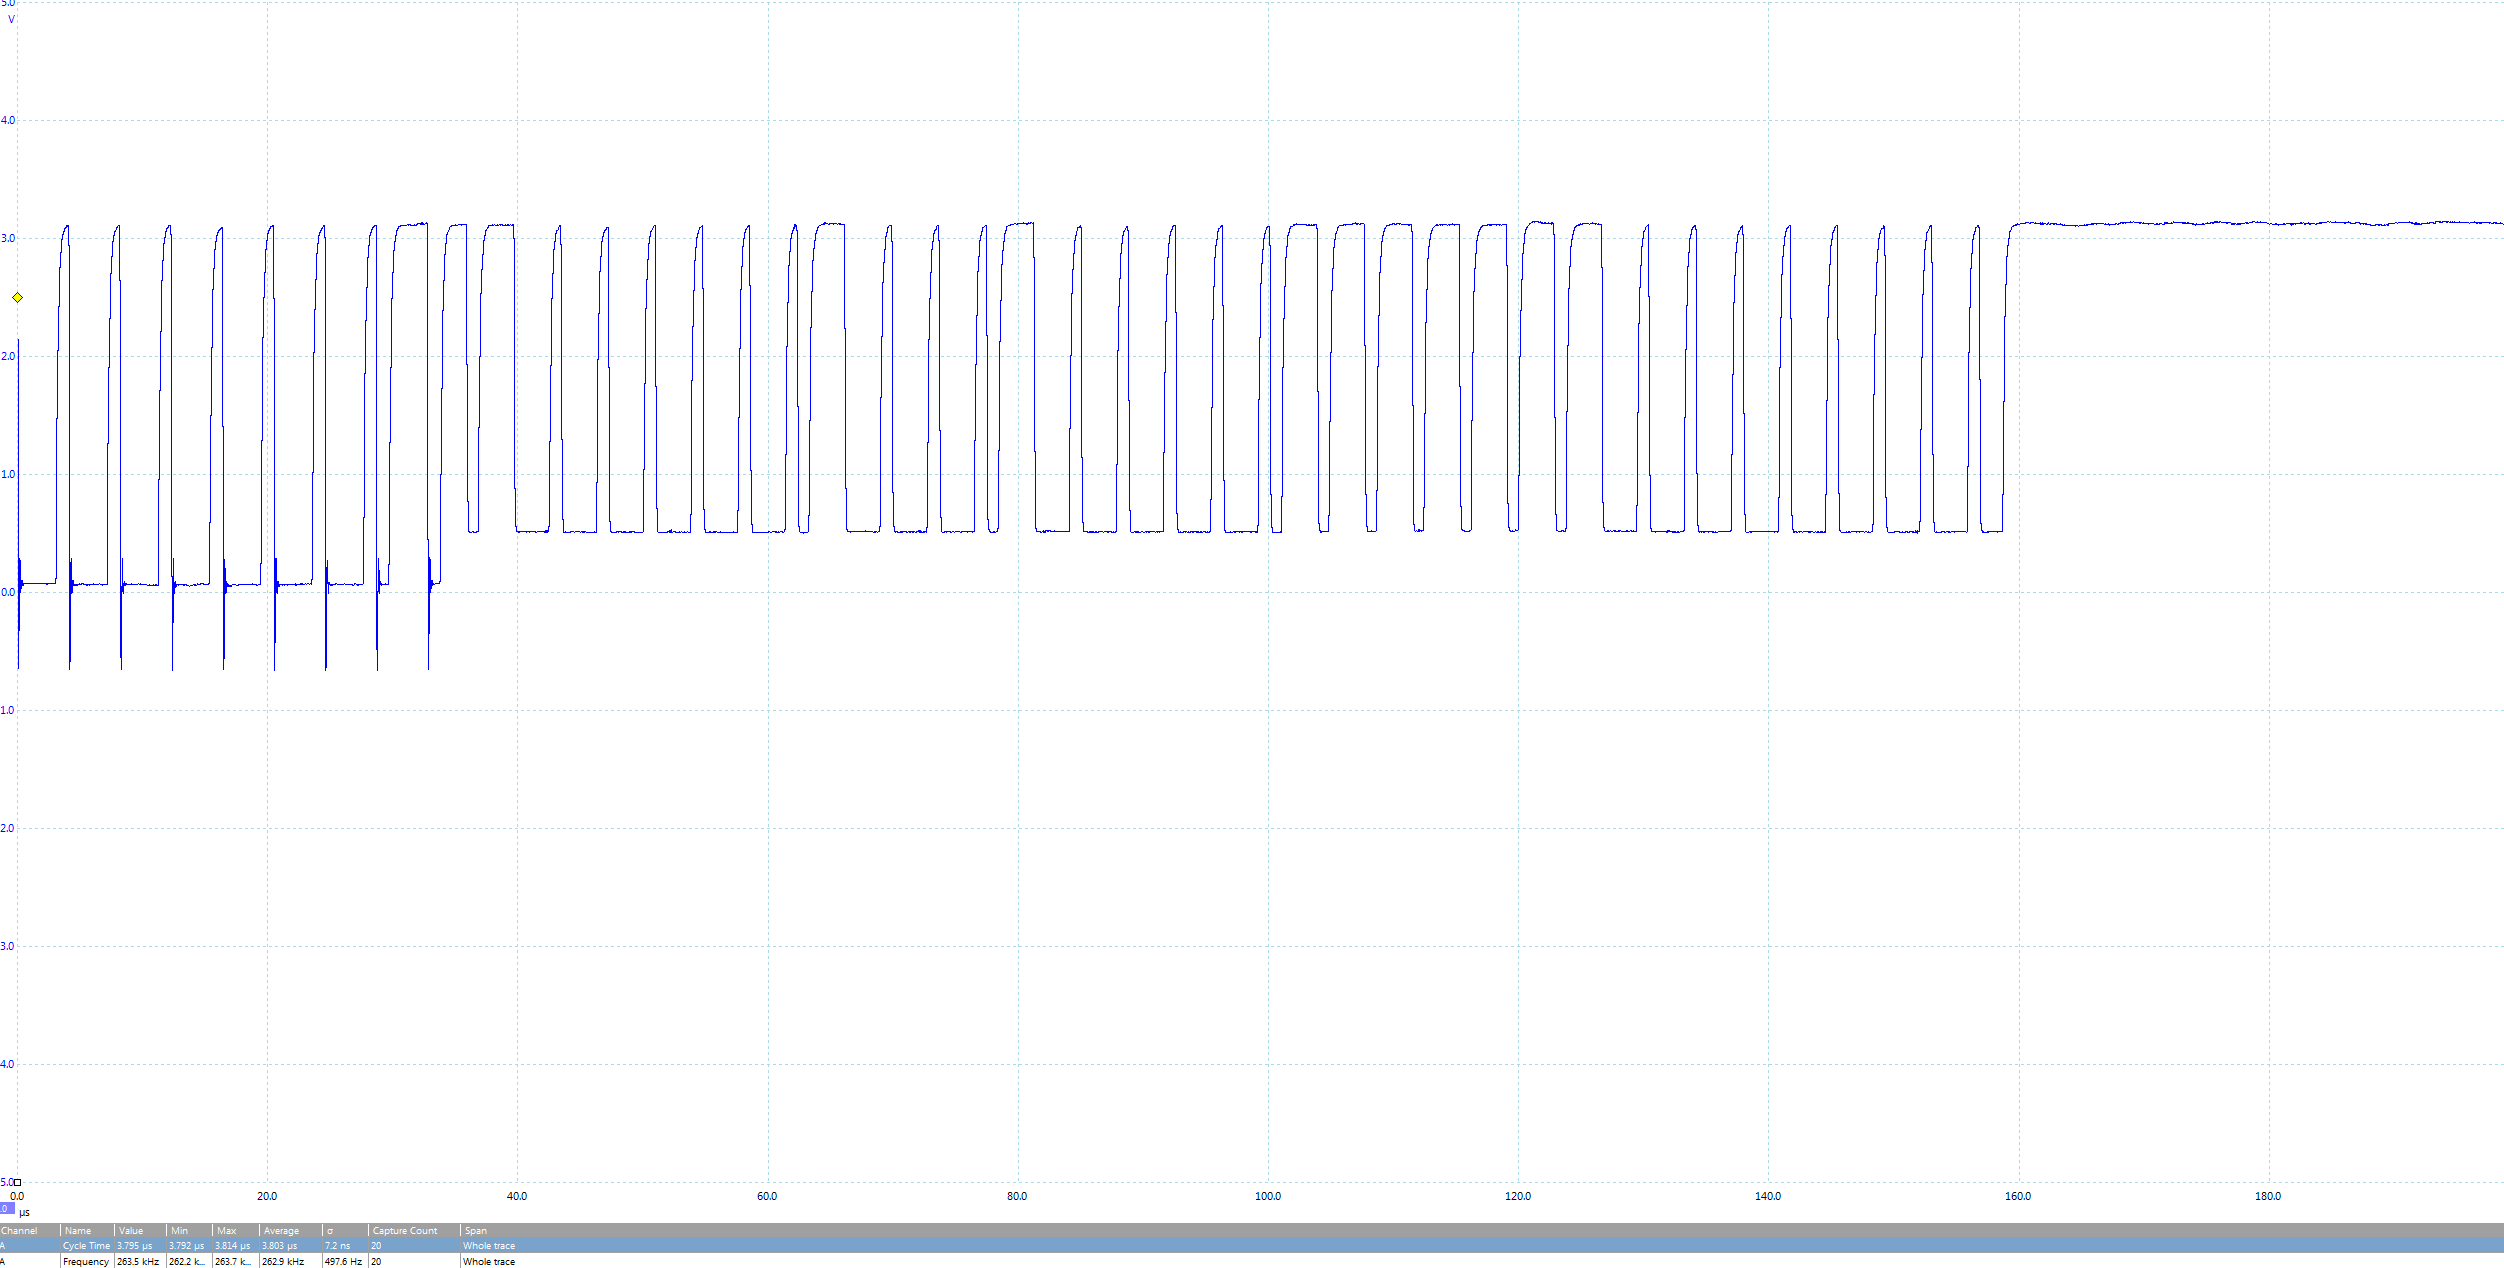
\includegraphics[width=\textwidth]{some_input.png}
  \caption{Input bits with some buttons pressed and stick tilted}
  \label{some_input}
\end{figure}

\subsection{Mupen64 movie files}
The file format read by the TASBot64 is that of Mupen64-rr, the version of the
Mupen64 emulator modified for the TAS purpose. The files usually take the .m64
extension.

At the beginning of the file is a simple fixed size header containing a magic
number to verify that the file is indeed of the right format, the format
version, whether the TAS was meant to be run with a game save or a snapshot, the
number of gamepads connected and the number of input frames (all numbers are
little endian). It also contains various metadata such as the name of the game
for which the TAS is made, the author of the TAS or a short description.

The input stream starts after the header, at address 0x400 in the file. It is a
serie of 4 bytes input frames, with the same bits layout as in the gamepad
protocol.

Since it is the console that chooses when it needs input, the input frames are
not tagged with any port number or timestamp : they are simply served, in order,
to any port that requests one.

\subsection{SD card}
The microcontroller will be attached to the SD card via the SPI (Serial Peripheral Interface) mode 0.

The structure of SPI is made of four signal lines: SCLK (Serial Clock), MISO (Master-In Slave-Out), MOSI (Master-Out Slave-In) and SS (Slave Select). Contents of both 8-bit shift register are exchanged with the shift clock driven by the master, SS will not be used since only one SD card will be used. In SPI mode, the data is transferred in byte oriented serial communication and it is based on SCLK timing.

The SPI mode 0 is one of the four possible timing mode allowed by the SPI and it is the one used by SD cards. This mode has the clock polarity (CPOL) set to zero, meaning that the base value (idle state) of the clock is 0, and the clock phase (CPHA) is set to zero as well, which tells to capture data on the clock's rising edge and to output data on a falling edge.

The commands (CMD) are given from the master to the slave with five or six bytes on the MOSI and then the master must continue reading on the MISO until a valid response is detected. The commands are always made up with the first byte stating the type (index) of command and the four following bytes giving all the arguments needed, there can be a final byte called CRC (cyclic redunndancy checking) which works as a check sum but this feature is optional in SPI mode. It must be remembered that the index byte always has the most left bit set to 0 and the following to 1, thus reducing the possible commands to 64 (from CMD0 to CMD63).

Depending on the command different types of response will come. The most common one is the R1 response which is a byte with its first bit to 0 and the following are flags set to 1 only if the related error happened (0x00 means succesful then). R3 and R7 response are made of an R1 plus 32 trailing bit data. Some commands may have the R1b response, which is a R1 followed by a busy flag. In that case MISO will be set to 0 and the microcontroller must wait until the SD card puts it back to 1 before giving further commands.

In a transaction with data transfer, one or more Data Blocks will be sent after command response. Each Data Block (which can be long up to 2048 bytes) is always preceded by a byte called Data Token (stating to which CMD it is responding) and it is always followed by a 2-bytes CRC, the sum of the three is called Data Packet. When a multiple block write transaction is finished a single byte called Stop Tran token is sent.

After a power-on or a reset SD cards enter their native operating mode, hence an initialization procedure must be launched each time one of this events happen in order tu put the card in SPI mode (otherwise only few CMD are accepted). First of all it must be checked that the system supply voltage is in the right working range (3.3 volts) otherwise the card must be rejected. Then, to actually start the initialization process, a CMD1 must be sent to the card and then the R1 response must be checked: if it corresponds to 0x01 then another CMD1 must be sent (and R1 response must be checked again and so on) while if it is equal to 0x00 the card is initialized properly.

\subsection{LCD display}
The display we will use, as the majority of LCD character mode displays, include
a Hitachi HD44780 compatible driver chip. This chip is talked to over a
Read/Write (R/W) pin, a Register Select (RS) pin, an 8 pin bus (DB[7..0]) and a
clock pin (E). Inside the chip are some configuration register and memory,
including an Address Counter (AC), a Display Data RAM (DDRAM) and a Character
Generator RAM (CGRAM).

In our case the R/W pin will stay low as we won't need to read back from the
chip. The CGRAM, whose purpose is to store custom characters, won't be used as
well. The chip also features a 4 bits mode, where DB[7..4] is used on two clock
fronts to provide one byte, which won't be used as well.

When RS is high, each falling edge on E write the byte given on DB[7..0] to
DDRAM, at the address stored in the internal register AC, that represents the
cursor position. AC is then incremented (or decremented, according to
configuration), so that the next character is written to the next posision on
the screen.

When RS is low, instead of character data, the byte on DB[7..0] is interpreted
as a command. These commands allow one to set the configuration, clear the
screen or set AC, among others. The variable length high part of the byte
specifies the command, while the low part is the argument.

Each command or memory write takes a defined time to process before another
action is possible, thus a delay of approximately \SI{40}{\us} is necessary
after each action. Refer to the datasheet for more details.

\section{Block diagram}

\section{Choice of components}
\subsection{MCU}
\subsubsection{CPU}
The gamepad protocol requires being ablo to flip a pin each \si{\us} at
most. With the lowest speed available (\SI{40}{\MHz}), that leaves us 40
instructions to decide what to do, which is enough. Console requests happen at
most each \SI{16}{\ms} and the whole exchange takes at most \SI{200}{\us}. We
then have $\SI{16}{\ms} - \SI{200}{\us} = \SI{15.8}{\ms}$ to do all the rest.

Writing to the screen (takes max \SI{6.4}{\ms} overall to fill the whole
screen) can largely be done in parallel to other tasks as it is mostly waiting
and it doesn't even need to be done every frame. All the remaining time can be
used to buffer data from the SD, and even that can probably offloaded in most
part to a DMA channel. So our CPU budget is plenty.

\subsubsection{Memory}

The smallest flash memory available is \SI{16}{\kibi\byte}. However if we look
at Microchip document AN1045, which is about using a library to access FAT32
filesystems, the Table 10 page 11 shows that their lib needs about
\SI{27}{\kibi\byte} of program memory. Moreover this table assumes a 16 bits CPU
while ours is 32 bits and probably has a more space-consuming instruction
set. While \SI{32}{\kibi\byte} may be sufficient (the PIC32 supports the MIPS16
reduced size instruction set), we choose to require \SI{64}{\kibi\byte} of
program memory to be on the safe side.

As a bonus, the \SI{64}{\kibi\byte} chips have more RAM, that can be used to
buffer more input frames and thus be less sensible to a low quality SD card with
long response times.

\subsubsection{Final choice}

To cater to our limited soldering capabilities, we are limited to a SDIP or
SOIC package.

The cheapest model meeting our requirements sold by our supplier is the
PIC32MX130F064B-I/SP. It is also available in a SOIC package but is more
expensive.

\subsection{Display}
We need to display the name of the game, which may be long and contain Japanese
characters, on one line, hence the longer the line the better. We need another
line to display the eventual error codes and progression of the TAS.

The display must also support a 3.3V electric supply and a backlight to indicate
the power-on status of the TASBot.

\section{Preliminary Bill of Materials}
\begin{tabular}{|l|l|l|l|l|}
  \hline
  Description & Qty & Producer & Producer ref & Supplier ref \\
  \hline
  PIC32 & 1 & Microchip & PIC32MX130F064B-I/SP & 2097776 \\
  \hline
  Display & 1 & Midas & MCCOG22005A6W-BNMLWI & 2218944 \\
  \hline
  SD card slot & 1 & Molex & 503182-1853 & 2334075 \\
  \hline
  Up and down buttons & 2 & & &\\
  \hline
  Passthrough switch & 1 & & &\\
  \hline
  Gamepad cable plugs & 4 & & &\\
  \hline
  UART connector & 1 & & &\\
  \hline
  RJ12 connector for ICD3 & 1 & Molex & 85513-5014 & 1388980 \\
  \hline
\end{tabular}

\section{Power consumption}
\begin{tabular}{|l|l|l|}
  \hline
  Component & Max current (\si{\mA}) \\
  \hline
  PIC32 & 300 \\
  \hline
  SD card & 100\\
  \hline
  Display & 0.2 \\
  \hline
  Display backlight & 50 \\
  \hline
  Total & 450.2\\
  \hline
\end{tabular}

\end{document}
